%!TEX root = edance.tex
%%%%%%%%%%%%%%%%
%  CHAPTER 16  %
%%%%%%%%%%%%%%%%
\chapter{Differential Amplifiers}
\label{ch:ch16_diff_amp}
\graphicspath{{./figures/figs_ch16_diffamp/}}
%%%%%%%%%%%%%%%%%%%%%%%%%%%%%%%%%%%%%%%%%%%%%%%%%%%%%%%%%%%%%%%%%%%%%%%%%%%%%%%%%%%%%%%%
%%%%%%%%%%%%%%%%%%%%%%%%%%%%%%%%%%%%%%%%%%%%%%%%%%%%%%%%%%%%%%%%%%%%%%%%%%%%%%%%%%%%%%%%
%                                   SECTION 16.1                                       %
%%%%%%%%%%%%%%%%%%%%%%%%%%%%%%%%%%%%%%%%%%%%%%%%%%%%%%%%%%%%%%%%%%%%%%%%%%%%%%%%%%%%%%%%
%%%%%%%%%%%%%%%%%%%%%%%%%%%%%%%%%%%%%%%%%%%%%%%%%%%%%%%%%%%%%%%%%%%%%%%%%%%%%%%%%%%%%%%%
\section{Chapter Preview}
This chapter introduces a very important building block known as the differential amplifier.  This amplifier is at the heart of almost every analog amplifier, and most notably forms the input stage of every operational amplifier (see \emph{Fig.~\ref{fig:ch16_intro}}).

We begin by motivating the need for differential amplifiers, and then we give a pseudo-historical account of how the differential amplifier was invented.  In this way we can actually learn how the amplifier takes form into a fully symmetric structure.  We will derive the transfer function in detail for both large and small signals.  The key to the analysis will be to take advantage of the symmetry in the circuit to simplify the analysis.  To do this, we need to take arbitrary inputs and represent it as a combination of \emph{differential-mode} and \emph{common-mode} signals, which enables us to make symmetry arguments.  With such a representation, we will define common-mode and differential-mode gains, and we will discuss important concepts such as common-mode rejection.

We end the chapter by discussing more advanced differential amplifier architectures, with current source and current mirror loads, which provide high gain and good common-mode rejection.
%%%%%%%%%%%%%%%%%%%%%%%%%%%%%%%%%%%%%%%%%%%%
%                 FIGURE                   %
%%%%%%%%%%%%%%%%%%%%%%%%%%%%%%%%%%%%%%%%%%%%
\begin{figure}[H]
\centering
\includegraphics[scale=0.35]{op_amp_diff}
\caption{In real op-amps there is always a non-zero voltage between the inputs.}
\label{fig:ch16_intro}
\end{figure}
%%%%%%%%%%%%%%%%%%%%%%%%%%%%%%%%%%%%%%%%%%%%
\newpage
%%%%%%%%%%%%%%%%%%%%%%%%%%%%%%%%%%%%%%%%%%%%
%                 FIGURE                   %
%%%%%%%%%%%%%%%%%%%%%%%%%%%%%%%%%%%%%%%%%%%%
\begin{figure}[t]
\centering
\includegraphics[scale=1.00]{diff_vs_cm} 
\caption{In a differential system, two wires carry the signal with opposite phase, as shown.  The differential signal is measured between the two wires.  In a single-ended system, only a single wire carries the signal and the potential is referenced to ground.}
\label{fig:diff_circ}
\end{figure}
%%%%%%%%%%%%%%%%%%%%%%%%%%%%%%%%%%%%%%%%%%%%
%                 FIGURE                   %
%%%%%%%%%%%%%%%%%%%%%%%%%%%%%%%%%%%%%%%%%%%%
\begin{figure}[H]
\centering
\includegraphics[scale=0.85]{diff_cm_noise} 
\caption{In a differential system, any noise pickup that is common-mode, for example from power supplies or from the substrate of the IC, is rejected since the output is a differential signal.  In a single-ended system, this noise cannot be distinguished from the signal itself.}
\label{fig:noise_reject}
\end{figure}
%%%%%%%%%%%%%%%%%%%%%%%%%%%%%%%%%%%%%%%%%%%%%%%%%%%%%%%%%%%%%%%%%%%%%%%%%%%%%%%%%%%%%%%%
%%%%%%%%%%%%%%%%%%%%%%%%%%%%%%%%%%%%%%%%%%%%%%%%%%%%%%%%%%%%%%%%%%%%%%%%%%%%%%%%%%%%%%%%
%                                   SECTION 16.2                                       %
%%%%%%%%%%%%%%%%%%%%%%%%%%%%%%%%%%%%%%%%%%%%%%%%%%%%%%%%%%%%%%%%%%%%%%%%%%%%%%%%%%%%%%%%
%%%%%%%%%%%%%%%%%%%%%%%%%%%%%%%%%%%%%%%%%%%%%%%%%%%%%%%%%%%%%%%%%%%%%%%%%%%%%%%%%%%%%%%%
\section{Motivation for Differential Operation}
First of all, what is a differential circuit?  In \emph{Fig.~\ref{fig:diff_circ}} we highlight the difference between a \textbf{"single-ended"} circuit\index{Single-ended circuit} and a \textbf{differential} circuit\index{Differential circuit}. In a single-ended circuit, \textit{all signals are referenced to a common ground}, and signals are routed using a single wire.  In a differential circuit, \textit{each signal is represented with two wires}.  Also, optimally each wire carries half of the signal such that each signal's phase is equal and opposite to the other.  In this form the signals are self-referenced without needing a ground connection.  The potential difference between the wires is known as the \textbf{differential-mode signal}\index{Differential-mode signal}.  The signal in common with both is known as the \textbf{common-mode signal}\index{Common-mode signal}.

Ideally the common-mode signal is just a DC reference or bias voltage, but in practice it may vary due to interference or imbalances.  A good example of interference is the ground or supply noise, that ideally couples to the differential wires in the same manner, producing a common-mode signal.  In a single-ended system, any common-mode noise is indistinguishable from the desired signal, and often it can swamp the desired signal.  A good example is the large AC voltages/currents flowing in power lines -- even a small fraction picked up by a sensor due to capacitive coupling can easily swamp out a micro-volt signal.  

Differential circuits are much less sensitive to common-mode noise and interference, and are preferred to the greatest extent possible.  As shown in \emph{Fig.~\ref{fig:noise_reject}}, common-mode noise is rejected in a differential circuit as long as the circuits are balanced (noise is picked up as a pure common mode signal).  Other benefits of the differential configuration is that it enables us to bias amplifiers and connect multiple stages without using coupling or bypass capacitors.  We will cover this in detail (see \emph{Fig.~\ref{fig:diff_amp_cascade}} later in this chapter).  

Correct differential operation requires excellent matching of transistors and other components.  This favors implementation in integrated circuit (IC) form, where matched transistors can be fabricated side-by-side or even inter-digitated together (see \emph{Fig.~\ref{fig:mirror_layout}}).  Differential amplifiers require twice as many transistors.  But again, in an IC this is not an issue at all, because transistors are essentially "free" compared to other larger components (such as resistors and capacitors).
%%%%%%%%%%%%%%%%%%%%%%%%%%%%%%%%%%%%%%%%%%%%%%%%%%%%%%%%%%%%%%%%%%%%%%%%%%%%%%%%%%%%%%%%
%%%%%%%%%%%%%%%%%%%%%%%%%%%%%%%%%%%%%%%%%%%%%%%%%%%%%%%%%%%%%%%%%%%%%%%%%%%%%%%%%%%%%%%%
%                                   SECTION 16.3                                       %
%%%%%%%%%%%%%%%%%%%%%%%%%%%%%%%%%%%%%%%%%%%%%%%%%%%%%%%%%%%%%%%%%%%%%%%%%%%%%%%%%%%%%%%%
%%%%%%%%%%%%%%%%%%%%%%%%%%%%%%%%%%%%%%%%%%%%%%%%%%%%%%%%%%%%%%%%%%%%%%%%%%%%%%%%%%%%%%%%
\section{Birth of Symmetric Source-Coupled Pair}
%%%%%%%%%%%%%%%%%%%%%%%%%%%%%%%%%%%%%%%%%%%%
%             SUBSECTION 16.3.1            %
%%%%%%%%%%%%%%%%%%%%%%%%%%%%%%%%%%%%%%%%%%%%
\subsection{Goal:  Differential Transconductance \texorpdfstring{$G_m$}{}}
Let's imagine that you're living in a pre-differential world where all signal processing is done in single-ended form.  You're inspired to build a transconductance stage that can be controlled by the difference in voltage between two nodes, rather than a single-ended transconductor, which is commonly used in the form of a transistor.  In other words, our goal is to have an output current that satisfies this equation:
    \begin{equation}
        i_o = G_m (v^+ - v^-)
    \end{equation}
Ideally the circuit should have very high output impedance and very little loading on nodes $v^+$ and $v^-$.  As a good circuit designer, you come to the realization that a common source and common gate amplifiers are complementary in the sense that they have opposite phase.  If you equalize the gain, you can potentially build a \textbf{differential transconductance}\index{Differential transconductance}, $G_m$.  In fact, you can combine the common source and common gate amplifier into a single transistor as shown in \emph{Fig.~\ref{fig:amp_diff_CS_CG}a}.  Let's calculate the gain by superposition.  If we excite $v^-$, and ground $v^+$, we have an output voltage given by:
    \begin{equation}
        v_{o,CS} = -g_m\,R_D\,v^-
    \end{equation} 
Likewise, if you excite the common gate stage through $v^+$ (and ground $v^-$), we have:
    \begin{equation}
        v_{o,CG} = g_m\,R_D\,v^+
    \end{equation} 
Summing these signals, we have:
    \begin{equation}
        v_o = g_m R_D(v^+ - v^-)
    \end{equation}
This looks pretty promising, so what's missing? 
\newpage
%%%%%%%%%%%%%%%%%%%%%%%%%%%%%%%%%%%%%%%%%%%%
%                 FIGURE                   %
%%%%%%%%%%%%%%%%%%%%%%%%%%%%%%%%%%%%%%%%%%%%
\begin{figure}[H]
\centering
\begin{tabular}{cc}
\includegraphics[scale=1.15]{amp_diff_CS_CG} &
\includegraphics[scale=1.15]{amp_diff_CS_CG_buffer}\\
(a) & (b)\\
\end{tabular}
\caption{(a) A combined common-gate and common source amplifier.  From the $v^+$ terminal, the circuit is a common gate amplifier, whereas from the $v^-$ terminal it is a common source amplifier.  (b) A buffer is needed to raise the impedance of the common gate amplifier if we wish to equalize the gain under arbitrary drive conditions.}
\label{fig:amp_diff_CS_CG}
\end{figure}
%%%%%%%%%%%%%%%%%%%%%%%%%%%%%%%%%%%%%%%%%%%%
%              SUB-SUBSECTION              %
%%%%%%%%%%%%%%%%%%%%%%%%%%%%%%%%%%%%%%%%%%%%
\subsubsection{Problem:  Asymmetric (Low) Input Impedance}
Notice that the gain is symmetric from the "plus" and "minus" side for an ideal voltage drive, but not for any drive with finite non-zero source resistance.  Because of the low input impedance of the common gate stage, there is going to be a gain mismatch.  This is due to the voltage division between the source $R_s$ and the input impedance of the common gate stage, which is roughly $\frac{1}{g_m}$:
    \begin{equation}
        v_{o,CG} = \left(\frac{\frac{1}{g_m}}{\frac{1}{g_m} + R_s}\right)\,g_m\,R_D\,v^+
        = \left(\frac{g_m}{1 + g_m\,R_s}\right)\,R_D\,v^+
    \end{equation}
%%%%%%%%%%%%%%%%%%%%%%%%%%%%%%%%%%%%%%%%%%%%
%              SUB-SUBSECTION              %
%%%%%%%%%%%%%%%%%%%%%%%%%%%%%%%%%%%%%%%%%%%%
\subsubsection{Solution:  Add Buffer to Source Side}
So what is the solution?  Simply adding a voltage buffer as shown in \emph{Fig.~\ref{fig:amp_diff_CS_CG}b} would solve the problem.  However, any real buffer has an output impedance, leading us back to the same issue.  For example, the source follower shown in \emph{Fig.~\ref{fig:amp_diff_CS_CG_CD}} has an output impedance of $\frac{1}{g_{m,buff}}$.  To minimize the voltage loss we could burn more and more power in the buffer to make the output impedance smaller.  But this is not an elegant solution, because the gain mismatch will always be there.
%%%%%%%%%%%%%%%%%%%%%%%%%%%%%%%%%%%%%%%%%%%%
%             SUBSECTION 16.3.2            %
%%%%%%%%%%%%%%%%%%%%%%%%%%%%%%%%%%%%%%%%%%%%
\subsection{Gain of Source Degenerated CS}
Let's think about this problem in another way.  The introduction of the buffer did not solve the problem completely, and in fact it introduced another problem.  Even though the input impedance of the common source stage is very large, the gain is now degenerated by the output impedance of the buffer:   
    \begin{equation}
        v_{o,CS} = -\left(\frac{g_m}{1 + g_m\left(\mathlarger{\frac{1}{g_{m,buff}}}\right)}\right)R_D\,v^-
    \end{equation}
What if we equalized the $g_{m,buff} = g_m$ with the common source/gate stage?  Then the gain loss for the common source would be $\frac{1}{2}$, and the buffer driving the common gate stage would also suffer a voltage loss of $\frac{1}{2}$.  In other words, in this symmetrical arrangement, the gains will be matched precisely as desired and both ports have a high input impedance.
\newpage
%%%%%%%%%%%%%%%%%%%%%%%%%%%%%%%%%%%%%%%%%%%%
%                 FIGURE                   %
%%%%%%%%%%%%%%%%%%%%%%%%%%%%%%%%%%%%%%%%%%%%
\begin{figure}[t]
\centering
\begin{tabular}{cc}
\includegraphics[scale=1.25]{amp_diff_CS_CG_CD} &
\includegraphics[scale=1.25]{amp_CG_CD_Model}\\
(a) & (b)\\
\end{tabular}
\caption{(a) Common source and common gate amplifier with a source follower buffer added.  (b) The buffer output impedance $\frac{1}{g_m}$ degenerates the common source stage, and reduces the gain of the common gate amplifier.}
\label{fig:amp_diff_CS_CG_CD}
\end{figure}
%%%%%%%%%%%%%%%%%%%%%%%%%%%%%%%%%%%%%%%%%%%%
%             SUBSECTION 16.3.3            %
%%%%%%%%%%%%%%%%%%%%%%%%%%%%%%%%%%%%%%%%%%%%
\subsection{A Symmetric Source Coupled Pair is Born}
Putting these ideas together, we arrive at \emph{Fig.~\ref{fig:amp_CS_CG_sym}a}.  The resistor $R_S$ is just there for biasing, and we can replace it with a current source and combine it with the current source of the follower.  The result, redrawn in \emph{Fig.~\ref{fig:amp_CS_CG_sym}b}, is a fully symmetric circuit.
%%%%%%%%%%%%%%%%%%%%%%%%%%%%%%%%%%%%%%%%%%%%
%                 FIGURE                   %
%%%%%%%%%%%%%%%%%%%%%%%%%%%%%%%%%%%%%%%%%%%%
\begin{figure}[H]
\centering
\begin{tabular}{cc}
\includegraphics[scale=1.2]{amp_CS_CG_sym} &
\includegraphics[scale=1.2]{amp_sym_pair}\\
(a) & (b)\\
\end{tabular}
\caption{(a) A combined common source and common gate amplifier with equally sized devices for the buffer and amplifier, thereby making the circuit symmetric.  (b) Redrawn circuit to emphasize the symmetry.  This circuit is known as the differential pair.}
\label{fig:amp_CS_CG_sym}
\end{figure}
%%%%%%%%%%%%%%%%%%%%%%%%%%%%%%%%%%%%%%%%%%%%
\newpage
The circuit in \emph{Fig.~\ref{fig:amp_CS_CG_sym}b} has two outputs, rather than one, which are in exactly the opposite phase.  The key insight is that the circuit is fully symmetric, and the gain from both sides is lowered by the same factor:
    \begin{equation}
        v_{o,CS} = -\frac{g_m}{1 + g_m\left(\frac{1}{g_m}\right)}\,R_D\,v^- = -\left(\frac{g_m}{2}\right)\,R_D\,v^-
    \end{equation}
    \begin{equation}
        v_{o,CG} = \frac{g_m}{1 + g_m\left(\frac{1}{g_m}\right)}\,R_D\,v^+ = +\left(\frac{g_m}{2}\right)\,R_D\,v+
    \end{equation}
For simplicity, we only consider one output, but there are in fact two outputs.  Because since they are opposite in phase, we can combine them and consider the output as the voltage difference between the drain nodes:
    \begin{equation}
        v_{o,1} = \left(\frac{g_m}{2}\right)\,R_D\,(v^+ - v^-)  
    \end{equation}
    \begin{equation}
        v_{o,2} = \left(\frac{g_m}{2}\right)\,R_D\,(v^- - v^+)  
    \end{equation}
In other words, we have a fully differential circuit, allowing us to carry the signal differentially at both the input and output:
    \begin{equation}
        v_{o,diff} = v_{o,1} - v_{o,2} = g_m\,R_D (v^+ - v^-) = g_m\,R_D\,v_{i,diff}  
    \end{equation}
\vspace{0.25cm}
%%%%%%%%%%%%%%%%%%%%%%%%%%%%%%%%%%%%%%%%%%%%
%                 FIGURE                   %
%%%%%%%%%%%%%%%%%%%%%%%%%%%%%%%%%%%%%%%%%%%%
\begin{figure}[H]
\centering
\includegraphics[scale=1.45]{diffamp_cm_dc}
\caption{Differential pair under a common mode DC voltage drive.}
\label{fig:diffamp_cm_dc}
\end{figure}
%%%%%%%%%%%%%%%%%%%%%%%%%%%%%%%%%%%%%%%%%%%%
\newpage
%%%%%%%%%%%%%%%%%%%%%%%%%%%%%%%%%%%%%%%%%%%%%%%%%%%%%%%%%%%%%%%%%%%%%%%%%%%%%%%%%%%%%%%%
%%%%%%%%%%%%%%%%%%%%%%%%%%%%%%%%%%%%%%%%%%%%%%%%%%%%%%%%%%%%%%%%%%%%%%%%%%%%%%%%%%%%%%%%
%                                   SECTION 16.4                                       %
%%%%%%%%%%%%%%%%%%%%%%%%%%%%%%%%%%%%%%%%%%%%%%%%%%%%%%%%%%%%%%%%%%%%%%%%%%%%%%%%%%%%%%%%
%%%%%%%%%%%%%%%%%%%%%%%%%%%%%%%%%%%%%%%%%%%%%%%%%%%%%%%%%%%%%%%%%%%%%%%%%%%%%%%%%%%%%%%%
\section{Differential Operation}
%%%%%%%%%%%%%%%%%%%%%%%%%%%%%%%%%%%%%%%%%%%%
%             SUBSECTION 16.4.1            %
%%%%%%%%%%%%%%%%%%%%%%%%%%%%%%%%%%%%%%%%%%%%
\subsection{MOS Differential Pair:  DC Bias}
Consider the differential pair with a DC bias connected to both sides of the input, as shown in \emph{Fig.~\ref{fig:diffamp_cm_dc}}.  We will shortly demonstrate that the DC bias point\index{DC bias point} of $M1$ and $M2$ does not depend on the common gate DC voltage, because the current source sets the bias point of each transistor at half the bias current $I_Q$:
    \begin{equation}
        I_{D_1} = I_{D_2} = \frac{I_Q}{2}
    \end{equation}
This must be true by a simple symmetry argument.  Everything is assumed to be symmetric, and so $I_Q$ must divide in half.  That means each transistor has the same $V_{GS}$, and consequently the same overdrive $V_{OD}$, assuming that the threshold voltages match:
    \begin{align}
        \frac{I_Q}{2} &= \frac{k_n}{2}{\left(V_{GS} - V_{T_n}\right)^2}\\[0.25cm]
        V_{GS_1} &= V_{GS_2} = {V_{T_n}} + \sqrt{\frac{I_Q}{k_n}} = V_{T_n} + V_{OD}
    \end{align}
The drain voltage for both transistors is also equal to:
    \begin{equation}
        V_{D_1} = V_{D_2} = V_{DD} - \left(\frac{I_Q}{2}\right)\,R_D
    \end{equation}
And the differential DC output is exactly zero:
    \begin{equation}
        V_{D_1} - V_{D_2} = 0\,V
    \end{equation}
Consequently, the DC level at the output is independent of DC level at input! In \emph{Fig.~\ref{fig:diff_amp_bias_cm}}, we illustrate this by varying the DC level at the input and finding the operating point in the circuit.  Clearly, the circuit operating point and the region of operation of $M1$ and $M2$ does not depend on the input DC level.  Note that although $V_{GS}$ and $V_{D}$ are held constant, the source voltage moves.  But since the source node is driven by an ideal current source, we can tolerate this variation.  This allows us to cascade differential pairs without worrying about DC level, which obviates the need for bulky AC coupling capacitors, as shown in \emph{Fig.~\ref{fig:diff_amp_cascade}}.  Is this too good to be true?  As long as we ensure that the current source is not squashed, the circuit works as advertised.  A real current source (transistor) has a finite headroom to operate, for example a $V_{OD}$ for a single transistor current source.
%%%%%%%%%%%%%%%%%%%%%%%%%%%%%%%%%%%%%%%%%%%%
%                 FIGURE                   %
%%%%%%%%%%%%%%%%%%%%%%%%%%%%%%%%%%%%%%%%%%%%
\begin{figure}[H]
\centering
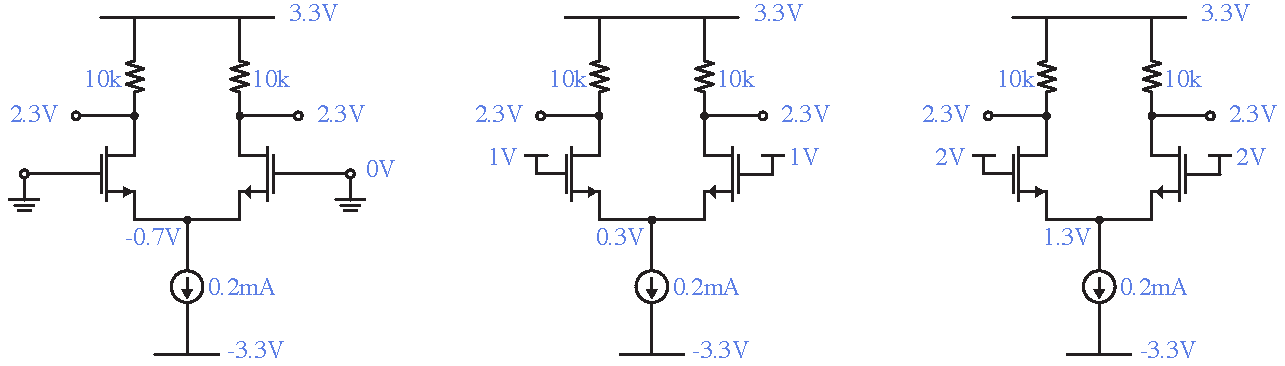
\includegraphics[width=\columnwidth]{diff_amp_bias_cm}
\caption{Differential pair with varying input DC voltage common-mode drive illustrating that the DC operating point of the circuit, in so far as the bias current and the drain voltage at the output is concerned, is independent of the input DC level.}
\label{fig:diff_amp_bias_cm}
\end{figure}
%%%%%%%%%%%%%%%%%%%%%%%%%%%%%%%%%%%%%%%%%%%%
\newpage
%%%%%%%%%%%%%%%%%%%%%%%%%%%%%%%%%%%%%%%%%%%%
%                 FIGURE                   %
%%%%%%%%%%%%%%%%%%%%%%%%%%%%%%%%%%%%%%%%%%%%
\begin{figure}[t]
\centering
\includegraphics[scale=1.05]{Diff_Cascade}
\caption{Cascading differential amplifiers without using AC coupling capacitors is possible because each amplifier bias point is independent of the input DC level, see \emph{Fig.~\ref{fig:diff_amp_bias_cm}}.}
\label{fig:diff_amp_cascade}
\end{figure}
%%%%%%%%%%%%%%%%%%%%%%%%%%%%%%%%%%%%%%%%%%%%
%                 FIGURE                   %
%%%%%%%%%%%%%%%%%%%%%%%%%%%%%%%%%%%%%%%%%%%%
\begin{figure}[H]
\centering
\includegraphics[scale=1.15]{Diffamp_large_signal}
\caption{Differential-Pair under arbitrary large signal drive at the inputs.}
\label{fig:Diff_amp_large}
\end{figure}
%%%%%%%%%%%%%%%%%%%%%%%%%%%%%%%%%%%%%%%%%%%%
%             SUBSECTION 16.4.2            %
%%%%%%%%%%%%%%%%%%%%%%%%%%%%%%%%%%%%%%%%%%%%
\subsection{MOS Differential-Pair:  Differential Inputs}
Let's consider applying a differential voltage to the differential pair as shown in \emph{Fig.~\ref{fig:Diff_amp_large}}.  We apply a gate voltage $v_1$ to $M1$ and $v_2$ to $M2$, with the condition that the difference between the inputs is the \textit{differential input signal}\index{Amplifier!differential amplifier!differential input signal}:
    \begin{equation}
        v_1 - v_2 = v_{id}
    \end{equation}
Since the input voltages applied to each gate is arbitrary, the current $I_Q$ no longer splits equally.  In fact, you can think of $M1$ and $M2$ as two devices competing for the current, $I_Q$.  The current will favor the device with higher $v_{GS}$.  So we can think of $M1$ and $M2$ as a pair of transistors that steer the current left or right, depending on the magnitude of the input drive.  For large positive voltage $v_{id} = v_{GS_1} - v_{GS_2}$, we expect most of the current $I_Q$ to be steered into $M1$.  Likewise, when $v_{id}$ is large and negative, then most of the current $I_Q$ should flow into $M2$.  Let's confirm this observation with the $MOS$ equations.  In general we have:
    \begin{align}
        i_{D_1} = \frac{k_n}{2}{\left(v_{GS_1} - V_T\right)^2}\\[0.15cm]
        i_{D_2} = \frac{k_n}{2}{\left(v_{GS_2} - V_T\right)^2}
    \end{align}
But the currents must sum to $I_Q$:
    \begin{equation}
        i_{D_1} + i_{D_2} = I_Q \rightarrow i_{D_2} = I_Q - i_{D_1}
    \end{equation}
Using these relations it is possible to derive a complete expression for the drain currents of $M1$ and $M2$ as a function of the differential voltage drive $v_{id}$:
    \begin{equation}
        i_{D_{1,2}} = \frac{I_Q}{2} \pm \sqrt{k_n\,I_Q} \left(\frac{v_{id}}{2}\right)
                        \sqrt{1 - \frac{{\mathlarger{\left(\frac{v_{id}}{2}\right)}}^2}{\mathlarger{\frac{I_Q}{k_n}}}}
    \end{equation}
Or in terms of the transistor overdrive voltage $V_{od}$, we know that the \textit{quiescent bias point}\index{Quiescent bias point} satisfies:
    \begin{equation}
        \frac{I_Q}{2} = \left(\frac{1}{2}\right)\,k_n\,{V_{OD}}^2 \;\longrightarrow\; k_n = \frac{I_Q}{{V_{OD}}^2}
    \end{equation}
Allowing us to express the current in the following insightful form:
    \begin{equation} 
        i_{D_{1,2}} = \frac{I_Q}{2} \pm \left(\frac{I_Q}{V_{OD}}\right) \left(\frac{v_{id}}{2}\right)
                        \sqrt{1 - \frac{{\mathlarger{\left(\frac{v_{id}}{2}\right)}}^2}{{V_{OD}}^2}}
        \label{eq:diff_large}
    \end{equation}
The full derivation is presented in \emph{Sec.~\ref{sec:derive_diff_large}} for your reference.  A plot of the currents through each transistor is shown in \emph{Fig.~\ref{fig:mosdiffamp_id}}.  As expected, the curves are symmetric with respect to the two transistors and the input voltage $v_{id}$, where a positive voltage $v_{id}$ steers the current into $M1$.  The steering is very linear near the origin, and if the input is sufficiently large, we see that the current is steered entirely in one direction or the other.  When $v_{id} = \sqrt{2}\,V_{OD}$, \emph{Eq.~\ref{eq:diff_large}} can be simplified:
    \begin{equation} 
        i_{D_{1,2}} = \frac{I_Q}{2} \pm \left(\frac{I_Q}{\cancel{V_{OD}}}\right) \left(\frac{\sqrt{2}\,\cancel{V_{OD}}}{2}\right)
                        \sqrt{1 - \frac{{\left(\frac{\sqrt{2}\,\bcancel{V_{OD}}}{2}\right)}^2}{{\bcancel{V_{OD}}}^2}}
                    = \frac{I_Q}{2} \pm \frac{I_Q}{2}
                    = \left\{\begin{array}{c c}
                        +I_Q & \to i_{D_1}\\
                        0 & \to i_{D_2}
                    \end{array}\right.
    \end{equation}
We see that all the current $I_Q$ goes to $i_{D1}$ when the input is sufficiently large and $M2$ shuts off.  When $v_{id} = -\sqrt{2}\,V_{OD}$, the situation is exactly the opposite, with $M1$ shutting off and $M2$ getting all the current $I_Q$.

The slope of the curves in \emph{Fig.~\ref{fig:mosdiffamp_id}} is the differential pair $G_m$ for each transistor.   The linear range of operation of the $MOS$ differential pair can be extended by operating the transistor at a higher value of $V_{OD}$, as shown in \emph{Fig.~\ref{fig:mosdiffamp_id_od}}.  At the origin, we can estimate the slope by considering a small input signal $v_{id}$, which causes the square root to be simplify:
    \begin{equation} 
        \sqrt{1 - \frac{{\mathlarger{\left(\frac{v_{id}}{2}\right)}}^2}{{V_{OD}}^2}} \approx 1
    \end{equation}
This results in linear deviations of the currents from the DC operation points:
    \begin{align} 
        i_{D_1} &= \frac{I_Q}{2} + \left(\frac{I_Q}{V_{OD}}\right) \left(\frac{v_{id}}{2}\right)\\
        i_{D_2} &= \frac{I_Q}{2} - \left(\frac{I_Q}{V_{OD}}\right) \left(\frac{v_{id}}{2}\right)
    \end{align}
It is clear that the first term is the bias current through $M1$ and $M2$.  The slope of the linear deviation is actually familiar.  It looks like the transistor $g_m$:
    \begin{equation}
        g_m = \frac{2\,I_D}{V_{OD}}
    \end{equation}
Since each transistor is biased at $\frac{I_Q}{2}$, the expression can be interpreted as follows:
    \begin{equation} 
        i_{D_{1,2}} = \frac{I_Q}{2} \pm \mathlarger{g_{m_{1,2}}} \left(\frac{v_{id}}{2}\right)
    \end{equation}
In other words, each transistor is excited in the small-signal with a voltage of $\frac{v_{id}}{2}$.  This is expected since the voltage $v_{id}$ is dropped across two series connected transistors (back-to-back), and the voltage splits in two.  What's surprising is that the $g_m$ looks like it is the transconductance of a common source stage, even though the source coupled node is "floating".  This requires some further explanation, provided next.
%%%%%%%%%%%%%%%%%%%%%%%%%%%%%%%%%%%%%%%%%%%%
%                 FIGURE                   %
%%%%%%%%%%%%%%%%%%%%%%%%%%%%%%%%%%%%%%%%%%%%
\begin{figure}[H]
\centering
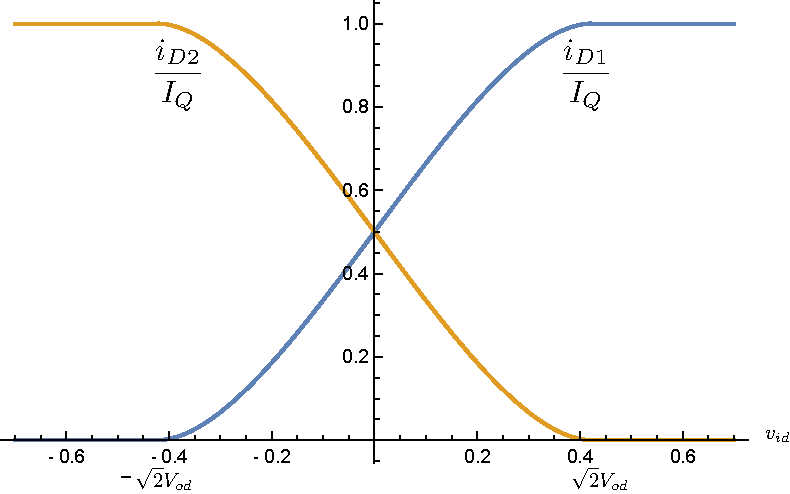
\includegraphics[scale=0.825]{mosdiffamp_id}
\caption{The currents in each branch of the differential pair circuit as a function of the input differential voltage $v_{id}$.  For zero drive, each transistor shares half of the current $I_Q$.  When the differential pair is steered with a voltage of $\pm \sqrt{2} V_{OD}$, the current switches completely to one branch.}
\label{fig:mosdiffamp_id}
\end{figure}
%%%%%%%%%%%%%%%%%%%%%%%%%%%%%%%%%%%%%%%%%%%%
%                 FIGURE                   %
%%%%%%%%%%%%%%%%%%%%%%%%%%%%%%%%%%%%%%%%%%%%
\begin{figure}[H]
\centering
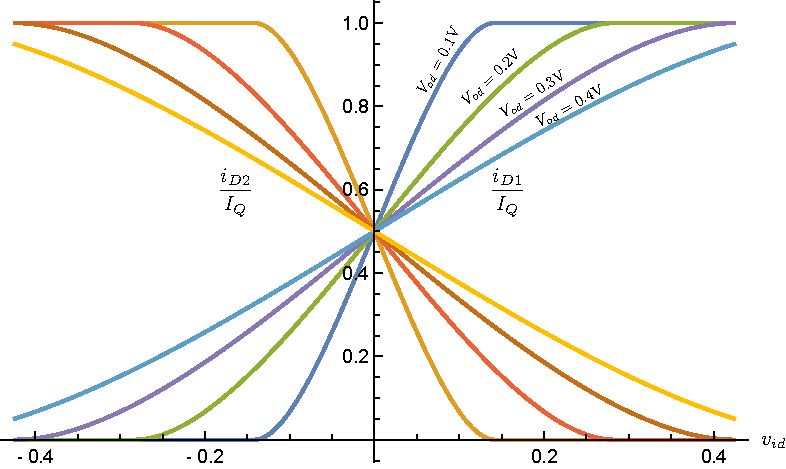
\includegraphics[scale=0.825]{mosdiffamp_id_od}
\caption{Family of currents in each branch of the differential pair circuit as a function of the input differential voltage $v_{id}$, with varying overdrive voltage $V_{OD}$.  Larger overdrive results in a larger linear range.}
\label{fig:mosdiffamp_id_od}
\end{figure}
%%%%%%%%%%%%%%%%%%%%%%%%%%%%%%%%%%%%%%%%%%%%
\newpage
%%%%%%%%%%%%%%%%%%%%%%%%%%%%%%%%%%%%%%%%%%%%
%                 FIGURE                   %
%%%%%%%%%%%%%%%%%%%%%%%%%%%%%%%%%%%%%%%%%%%%
\begin{figure}[t]
\centering
\includegraphics[scale=1.25]{Diff_Pair_Diff_CM}
\caption{The differential pair driven with both a common-mode and differential mode signal.}
\label{fig:Diff_Pair_Diff_CM}
\end{figure}
%%%%%%%%%%%%%%%%%%%%%%%%%%%%%%%%%%%%%%%%%%%%%%%%%%%%%%%%%%%%%%%%%%%%%%%%%%%%%%%%%%%%%%%%
%%%%%%%%%%%%%%%%%%%%%%%%%%%%%%%%%%%%%%%%%%%%%%%%%%%%%%%%%%%%%%%%%%%%%%%%%%%%%%%%%%%%%%%%
%                                   SECTION 16.5                                       %
%%%%%%%%%%%%%%%%%%%%%%%%%%%%%%%%%%%%%%%%%%%%%%%%%%%%%%%%%%%%%%%%%%%%%%%%%%%%%%%%%%%%%%%%
%%%%%%%%%%%%%%%%%%%%%%%%%%%%%%%%%%%%%%%%%%%%%%%%%%%%%%%%%%%%%%%%%%%%%%%%%%%%%%%%%%%%%%%%
\section{Small-Signal Differential Circuits}
%%%%%%%%%%%%%%%%%%%%%%%%%%%%%%%%%%%%%%%%%%%%
%             SUBSECTION 16.5.1            %
%%%%%%%%%%%%%%%%%%%%%%%%%%%%%%%%%%%%%%%%%%%%
\subsection{General Differential Drive}
The key to analyzing differential circuits is to apply a general input to the amplifier with voltages $v_1$ and $v_2$, and express it as a combination of a \textit{"common-mode" signal}\index{Common-mode signal} $v_{CM}$, and a \textit{"differential-mode" signal}\index{Differential-mode signal} $v_{DM}$:
    \begin{align}
        v_1 &= v_{CM} + \frac{v_{DM}}{2}
        \label{eq:v1}\\[0.15cm]
        v_2 &= v_{CM} - \frac{v_{DM}}{2}
        \label{eq:v2}
    \end{align}
To find $v_{CM}$, sum the signals so that $v_{DM}$ cancels out:
    \begin{equation}
        v_1 + v_2 = 2\,v_{CM}
        \label{eq:diff_combo}
    \end{equation}
\emph{Eq.~\ref{eq:diff_combo}} shows that $v_{CM}$ is the average input to the amplifier:
    \begin{equation}
        v_{CM} = \frac{v_1 + v_2}{2}
    \end{equation}
Next, take the difference between \emph{Eq.~\ref{eq:v1}} and \emph{Eq.\ref{eq:v2}} to cancel out $v_{CM}$:
    \begin{equation}
        v_1 - v_2 = v_{DM} 
        \label{eq:diff_combo_2}
    \end{equation}
Putting \emph{Eq.~\ref{eq:diff_combo}} and \emph{Eq.~\ref{eq:diff_combo_2}} together, we can form a system of equations:
    \begin{equation}
    	\left[\begin{matrix}
    		v_{CM}\\[0.1cm]
    		v_{DM}
    	\end{matrix}\right]
    	=
    	\left[\begin{matrix}
    		+\frac{1}{2} & +\frac{1}{2}\\[0.1cm]
    		+1 & -1
    	\end{matrix}\right]
    	\cdot
    	\left[\begin{matrix}
    		v_{1}\\[0.1cm]
    		v_{2}
    	\end{matrix}\right]
    \end{equation}  
These set of transformations are invertible, and one can go back and forth between the two representations.  You can verify by matrix inversion that we can reconstruct our original signals:
    \begin{equation}
    	\left[\begin{matrix}
    		v_{1}\\[0.1cm]
    		v_{2}
    	\end{matrix}\right]
    	=
    	\left[\begin{matrix}
    		+1 & +\frac{1}{2}\\[0.1cm]
    		+1 & -\frac{1}{2}
    	\end{matrix}\right]
    	\cdot
    	\left[\begin{matrix}
    		v_{CM}\\[0.1cm]
    		v_{DM}
    	\end{matrix}\right]
    \end{equation}  
The reason we prefer to represent our signal in terms of a "common-mode" and "differential-mode" is due to the symmetry of the waveforms, $v_{CM}$ and $v_{DM}$.  Since the differential pair is fully symmetric, applying a "common-mode" signal has "even" symmetry.  The left and right side of the circuit are excited with the same signal, so we expect the circuit to respond in the same way on the left and right hand sides.  On the other hand, exciting a circuit with $v_{DM}$ has "odd" symmetry, because every signal on the left should be the polar opposite of what is on the right.	Finally, as discussed earlier, the differential signal is usually of interest, and we typically want to amplify this component of the signal. The AC portion of the common-mode signal is interference or noise, and it should be rejected.  
%%%%%%%%%%%%%%%%%%%%%%%%%%%%%%%%%%%%%%%%%%%%
%                 FIGURE                   %
%%%%%%%%%%%%%%%%%%%%%%%%%%%%%%%%%%%%%%%%%%%%
\begin{figure}[t]
\centering
\includegraphics[width=\columnwidth]{DM_model}
\caption{AC circuit schematic of a symmetric circuit driven by a pure differential signal.  Since the common source node does not move, it can be grounded without changing the behavior of the circuit.}
\label{fig:DM_model}
\end{figure}
%%%%%%%%%%%%%%%%%%%%%%%%%%%%%%%%%%%%%%%%%%%%
%             SUBSECTION 16.5.2            %
%%%%%%%%%%%%%%%%%%%%%%%%%%%%%%%%%%%%%%%%%%%%
\subsection{Pure Differential-Mode Excitation}
To take a concrete example, consider the circuit shown in \emph{Fig.~\ref{fig:DM_model}}. When the inputs are purely differential-mode, the middle "source" node does not experience any voltage fluctuation.  This is true even if the source node has a finite impedance to ground.  Due to superposition, we can say that any fluctuation induced from one side of the differential pair is canceled by the other side due to the symmetry. Therefore, we are free to place a "virtual" ground at this node and split the circuit in two, with a grounded source connection.  Note that we have created a virtual ground without using a large bypass capacitor!  Now you may appreciate why the large-signal analysis of the previous section resulted in a small-signal $g_m$ that corresponded to a common source amplifier without degeneration.
%%%%%%%%%%%%%%%%%%%%%%%%%%%%%%%%%%%%%%%%%%%%
%             SUBSECTION 16.5.3            %
%%%%%%%%%%%%%%%%%%%%%%%%%%%%%%%%%%%%%%%%%%%%
\subsection{Pure Common-Mode Excitation}
Now consider the circuit shown in \emph{Fig.~\ref{fig:CM_model}}.  When the inputs are purely common-mode, then by symmetry no current can flow from the "left" to "right", because all of the signals are in phase.  Thus, we are free to cut this node and split the circuit into two identical circuits.  Note that the common-mode half circuit differs from the differential-mode half circuit, as one is grounded while the other one is "floating".  This leads to different values of common-mode and differential-mode gain.
%%%%%%%%%%%%%%%%%%%%%%%%%%%%%%%%%%%%%%%%%%%%
%                 FIGURE                   %
%%%%%%%%%%%%%%%%%%%%%%%%%%%%%%%%%%%%%%%%%%%%
\begin{figure}[H]
\centering
\includegraphics[width=\columnwidth]{CM_model}
\caption{AC circuit schematic of a symmetric circuit driven by a pure common-mode signal.  Since no current can travel through the middle branch, it can be cut without changing the behavior of the circuit.}
\label{fig:CM_model}
\end{figure}
%%%%%%%%%%%%%%%%%%%%%%%%%%%%%%%%%%%%%%%%%%%%
\newpage
%%%%%%%%%%%%%%%%%%%%%%%%%%%%%%%%%%%%%%%%%%%%
%                 FIGURE                   %
%%%%%%%%%%%%%%%%%%%%%%%%%%%%%%%%%%%%%%%%%%%%
\begin{figure}[t]
\centering
\includegraphics[scale=1.05]{Diff_Pair_DM_Drive}
\caption{AC model of a differential pair under pure differential drive.   The circuit can be split into two common-source amplifiers.}
\label{fig:Diff_Pair_DM_Drive}
\end{figure}
%%%%%%%%%%%%%%%%%%%%%%%%%%%%%%%%%%%%%%%%%%%%
%                 FIGURE                   %
%%%%%%%%%%%%%%%%%%%%%%%%%%%%%%%%%%%%%%%%%%%%
\begin{figure}[H]
\centering
\includegraphics[scale=1.35]{Diff_ss_gain}
\caption{Schematic of the differential circuit biased with a DC voltage $V_{CM}$ and driven with a pure differential drive.}
\label{fig:Diff_ss_gain}
\end{figure}
%%%%%%%%%%%%%%%%%%%%%%%%%%%%%%%%%%%%%%%%%%%%
%             SUBSECTION 16.5.4            %
%%%%%%%%%%%%%%%%%%%%%%%%%%%%%%%%%%%%%%%%%%%%
\subsection{Differential-Mode "Half Circuit"}
Under differential-mode excitation, we now analyze each half of the pair independently.  The circuit has been split into two, and each half is a simple CS amplifier, as shown in \emph{Fig.~\ref{fig:Diff_Pair_DM_Drive}}.
%%%%%%%%%%%%%%%%%%%%%%%%%%%%%%%%%%%%%%%%%%%%
%              SUB-SUBSECTION              %
%%%%%%%%%%%%%%%%%%%%%%%%%%%%%%%%%%%%%%%%%%%%
\subsubsection{Differential-Mode Gain}
The first step in analyzing any AC circuit is to find the DC operating point.  Seen in \emph{Fig.~\ref{fig:Diff_ss_gain}}, each transistor is biased at $\frac{I_Q}{2}$, with the gates at a common DC bias of $V_{CM}$.  Note that the common-mode signal is DC, and not AC.:
    \begin{equation}
        v_{G1.2} = V_{CM} \pm \left(\frac{1}{2}\right)\,v_{DM}
    \end{equation}
The AC circuit it is excited by a pure differential-mode signal, and given by:
    \begin{equation}
        v_{g1.2} = \pm \left(\frac{1}{2}\right)\,v_{DM}
    \end{equation}
The output at the $\pm$ nodes is:
    \begin{align}
        {v_o}^- &= -g_m\left(\frac{{v_{DM}}}{2}\right){R_D} = -g_m\,R_D\,\frac{{v_{DM}}}{2}\\[0.2cm]
        {v_o}^+ &= -g_m\left(-\frac{{v_{DM}}}{2}\right){R_D} = g_m\,R_D\,\frac{{v_{DM}}}{2}
    \end{align}
The differential output is the voltage $v_o = v_o^+ - v_o^-$, which leads to a differential-mode gain of:
    \begin{align} 
        \Aboxed{A_d &= \frac{{{v_{o}^+} - {v_{o}^-}}}{{{v_{DM}}}} = {g_m}{R_D}}
        &\textit{Differential-mode gain}
        \label{eq:diff_mode_gain}
    \end{align}
%%%%%%%%%%%%%%%%%%%%%%%%%%%%%%%%%%%%%%%%%%%%
%             SUBSECTION 16.5.5            %
%%%%%%%%%%%%%%%%%%%%%%%%%%%%%%%%%%%%%%%%%%%%
\subsection{Complete Small-Signal Differential and Common-Mode Models}
The complete small-signal models for differential-mode and common-mode operation are shown in \emph{Fig.~\ref{fig:DM_symmetry_small_signal}} and \emph{Fig.~\ref{fig:CM_symmetry_small_signal}}.  For the differential-mode circuit, since the schematic is split in the middle, we just have a common source amplifier.  So everything we have learned about CS amplifiers can be transferred to the differential pair.  We have been implicitly using these small-signal models in our analysis thus far.  For the common-mode equivalent half circuit, it is noteworthy that the circuit is "floating", and thus it cannot process any signals.  To see this, note that when a voltage is applied to the gate of one side, the source node will simply follow to ensure that $v_{gs} = 0\,V$.  So the output current of the transistor is zero, effectively rejecting the common-mode signal.  As far as the source node is considered, the circuit is a source follower after all.  Without modeling the impedance of a current source, the common-mode rejection is infinite.
%%%%%%%%%%%%%%%%%%%%%%%%%%%%%%%%%%%%%%%%%%%%
%                 FIGURE                   %
%%%%%%%%%%%%%%%%%%%%%%%%%%%%%%%%%%%%%%%%%%%%
\begin{figure}[H]
\centering
\includegraphics[width=\columnwidth]{DM_symmetry_small_signal}
\caption{Small-signal AC schematic of a differential pair excited with a differential signal.}
\label{fig:DM_symmetry_small_signal}
\end{figure}
%%%%%%%%%%%%%%%%%%%%%%%%%%%%%%%%%%%%%%%%%%%%
%                 FIGURE                   %
%%%%%%%%%%%%%%%%%%%%%%%%%%%%%%%%%%%%%%%%%%%%
\begin{figure}[H]
\centering
\includegraphics[width=\columnwidth]{CM_symmetry_small_signal}
\caption{Small-signal AC schematic of a differential pair excited with a common-mode signal.}
\label{fig:CM_symmetry_small_signal}
\end{figure}
%%%%%%%%%%%%%%%%%%%%%%%%%%%%%%%%%%%%%%%%%%%%
\newpage
%%%%%%%%%%%%%%%%%%%%%%%%%%%%%%%%%%%%%%%%%%%%
%                 FIGURE                   %
%%%%%%%%%%%%%%%%%%%%%%%%%%%%%%%%%%%%%%%%%%%%
\begin{figure}[t]
\centering
\begin{tabular}{cc}
\includegraphics[scale=1]{Diff_Pair_CM_inputs} &
\includegraphics[scale=1]{Diff_Pair_AC_SS}\\
(a) & (b)\\
\end{tabular}
\caption{(a) A differential pair with a real current source must include the current source output impedance. (b) The AC circuit can be split in half due to symmetry.  Splitting a resistor in half in the parallel direction is equivalent to two resistors in parallel, each with twice the resistance.}
\label{fig:Diff_Pair_CM_inputs}
\end{figure}
%%%%%%%%%%%%%%%%%%%%%%%%%%%%%%%%%%%%%%%%%%%%
%             SUBSECTION 16.5.6            %
%%%%%%%%%%%%%%%%%%%%%%%%%%%%%%%%%%%%%%%%%%%%
\subsection{Common-Mode Operation - Real Current Source}
The modified differential pair, shown in \emph{Fig.~\ref{fig:Diff_Pair_CM_inputs}a}, uses a real current source, with $R_{CS}$ modeling the output impedance of the current source.  By splitting $R_{CS}$ in two parallel resistors $2R_{CS}$, the circuit is fully symmetric.  This symmetry allows the half-circuit decomposition shown in \emph{Fig.~\ref{fig:Diff_Pair_CM_inputs}b}.  Now, the source is no longer floating, meaning that common-mode signals will see a (small) gain.  The gain can be made arbitrarily small by increasing $R_{CS}$ relative to $R_D$, but lowering $R_D$ also hurts the differential-mode gain.  We need to consider both to understand how well a circuit can amplify differential signals while rejecting common-mode signals.
%%%%%%%%%%%%%%%%%%%%%%%%%%%%%%%%%%%%%%%%%%%%
%             SUBSECTION 16.5.7            %
%%%%%%%%%%%%%%%%%%%%%%%%%%%%%%%%%%%%%%%%%%%%
\subsection{Differential and Common-Mode Gain}
Obviously, the most important gain is the differential-mode gain:
    \begin{equation}
        A_{DM} = \frac{v_{o_{DM}}}{v_{i_{DM}}}
    \end{equation}
Also of concern, is the common-mode gain, because a common-mode signal could potentially "jam" the amplifier by causing it to rail:
    \begin{equation}
        A_{CM} = \frac{v_{o_{CM}}}{v_{i_{CM}}}
    \end{equation}
Notice that it is entirely possible for a common-mode signal to be converted to a differential-mode through any kind of imbalances or mismatches in the amplifier.  This is especially problematic, because when this conversion occurs, the common-mode signal is indistinguishable from the differential-mode.  Thus, we would like to minimize:
    \begin{equation}
        A_{CM \to DM} = \frac{v_{o_{DM}}}{v_{i_{CM}}}
    \end{equation}
In a fully balanced amplifier, with differential inputs and outputs and zero mismatch between the components, $A_{CM \to DM}$ is identically zero.  But when the output is unbalanced (only one output is taken), or if there are mismatches between components, $A_{CM \to DM}$ can be of great importance.  Finally, even though it is possible to convert differential-mode to common-mode, this is usually of less concern.  
%%%%%%%%%%%%%%%%%%%%%%%%%%%%%%%%%%%%%%%%%%%%
%             SUBSECTION 16.5.8            %
%%%%%%%%%%%%%%%%%%%%%%%%%%%%%%%%%%%%%%%%%%%%
\subsection{Small-Signal Common-Mode Operation}
Let's analyze \emph{Fig.~\ref{fig:Diff_Pair_CM_inputs}b}.  Recall that $R_{CS}$ models any output resistance at the common-source node to ground.  The gain in common-mode is simply the gain of a source degenerated amplifier:
    \begin{equation}
        A_{CM} = -\left(\frac{g_m}{1 + g_m\,2\,R_{CS}}\right)R_D \approx -\frac{R_D}{2\,R_{CS}}
    \end{equation}
If we examine the differential output, the signal is zero (assuming perfect matching):
    \begin{equation}
        A_{CM \to DM} = 0
    \end{equation}
%%%%%%%%%%%%%%%%%%%%%%%%%%%%%%%%%%%%%%%%%%%%
%                 FIGURE                   %
%%%%%%%%%%%%%%%%%%%%%%%%%%%%%%%%%%%%%%%%%%%%
\begin{figure}[t]
\centering
\begin{tabular}{cc}
\includegraphics[scale=1.00]{Diff_mirror_load} &
\includegraphics[scale=1.00]{Diff_mirror_cascode}\\
(a) & (b)\\
\end{tabular}
\caption{(a) Differential pair with a current mirror load.  (b) A cascode differential pair with a cascode load.}
\label{fig:Diff_mirror_load}
\end{figure}
%%%%%%%%%%%%%%%%%%%%%%%%%%%%%%%%%%%%%%%%%%%%
%             SUBSECTION 16.5.9            %
%%%%%%%%%%%%%%%%%%%%%%%%%%%%%%%%%%%%%%%%%%%%
\subsection{Current-Source Loads}
Similar to a common source amplifier, an \textbf{active load}\index{Amplifier!active load} is often preferred.  Active loads occupy less area and require less headroom\index{Amplifier!headroom}.  The differential-mode gain with the active current source loads in \emph{Fig.~\ref{fig:Diff_mirror_load}a} is simply given by:
    \begin{equation}
        A_{DM} = \frac{v_{o_{DM}}}{v_{i_{DM}}} = g_{m,1}\,\left(r_{o,1} \parallel r_{o,3}\right)
    \end{equation}
To increase the gain, at the expense of loss of swing\index{Voltage swing}, we can \textit{cascode the load}\index{Amplifier!cascode loading}.  To reap the benefits of the higher output impedance of the load, we have to convert the differential pair into a \textbf{cascode differential pair}\index{Amplifier!cascode differential pair} to boost the output impedance:
    \begin{equation}
        A_{DM} = \frac{v_{o_{DM}}}{v_{i_{DM}}} = g_{m,1}\,\left(R_{on} \parallel R_{op}\right)
    \end{equation}
From our knowledge of cascodes, we can estimate the impedance seen looking into the $NMOS$ transistors:
    \begin{equation}
        R_{on} = \left(g_{m,3}\,r_{o,3}\right)\,r_{o,1}
    \end{equation}
And likewise the $PMOS$ load transistors:
    \begin{equation}
        R_{op} = \left(g_{m,5}\,r_{o,5}\right)\,r_{o,7}
    \end{equation}
The overall output impedance is the parallel combination.  For simplicity, assume the $NMOS$ and $PMOS$ loads present equal load impedance:
    \begin{equation}
        R_{on} = R_{op} = g_m\,{r_o}^2
    \end{equation}
This means the maximum differential-mode gain is given by:
    \begin{equation}
        A_{DM} = \left(\frac{1}{2}\right)\,{g_m}^2\,{r_o}^2
    \end{equation}
We can boost the gain higher by using a triple cascode, but the loss of headroom is unacceptable for most applications.
%%%%%%%%%%%%%%%%%%%%%%%%%%%%%%%%%%%%%%%%%%%%%%%%%%%%%%%%%%%%%%%%%%%%%%%%%%%%%%%%%%%%%%%%
%%%%%%%%%%%%%%%%%%%%%%%%%%%%%%%%%%%%%%%%%%%%%%%%%%%%%%%%%%%%%%%%%%%%%%%%%%%%%%%%%%%%%%%%
%                                   SECTION 16.6                                       %
%%%%%%%%%%%%%%%%%%%%%%%%%%%%%%%%%%%%%%%%%%%%%%%%%%%%%%%%%%%%%%%%%%%%%%%%%%%%%%%%%%%%%%%%
%%%%%%%%%%%%%%%%%%%%%%%%%%%%%%%%%%%%%%%%%%%%%%%%%%%%%%%%%%%%%%%%%%%%%%%%%%%%%%%%%%%%%%%%
\section{Common-Mode Rejection Ratio and DC Offsets}
\label{sec:cmrr}
%%%%%%%%%%%%%%%%%%%%%%%%%%%%%%%%%%%%%%%%%%%%
%             SUBSECTION 16.6.1            %
%%%%%%%%%%%%%%%%%%%%%%%%%%%%%%%%%%%%%%%%%%%%
\subsection{Common-Mode Rejection Ratio}
As we have emphasized, an important metric for a differential amplifier is its ability to reject the common-mode signal relative to the differential-mode signal.  The ratio of the gain is known as the \textbf{common-mode rejection ratio}\index{Common-mode rejection ratio} $CMRR$:
    \begin{align} 
        \Aboxed{CMRR &\equiv \frac{\left|A_{DM}\right|}{\left|A_{CM \to DM}\right|}}
        &\textit{Common-mode rejection ratio}
        \label{eq:cmrr_definition}
    \end{align}
Notice that an ideal (matched) amplifier has zero $A_{CM \to DM}$, and so it has an infinite $CMRR$. Certain applications, such as sensitive biomedical measurements require $70\,dB$ - $100\,dB$ of $CMRR$ to reject environmental noise (such as $50$/$60$ $Hz$ AC power) compared to minuscule sensor signals!
%%%%%%%%%%%%%%%%%%%%%%%%%%%%%%%%%%%%%%%%%%%%
%             SUBSECTION 16.6.2            %
%%%%%%%%%%%%%%%%%%%%%%%%%%%%%%%%%%%%%%%%%%%%
\subsection{Common-Mode Gain with Mismatched \texorpdfstring{$R_D$}{Load Resistance}}
Suppose we have a mismatch in the load resistors.  Then the gain from one side of the amplifier will not match the gain from the other side, causing the common-mode signal to be converted to differential-mode.  Let's say one resistor is larger by $\Delta\,R_{D}$:
    \begin{equation} 
        R_{D_{1,2}} = R_D \pm \frac{\Delta\,R_D}{2}
    \end{equation}
Now calculate the differential-mode output for a common-mode input:
    \begin{equation}
        v_{o_{DM}} = v_{o,2} - v_{o,1} = \frac{-\Delta\,R_D}{2\,R_{CS}}v_{i_{CM}}
    \end{equation}
This leads to \textit{common-mode to differential-mode gain}:
    \begin{equation} 
        A_{CM \to DM} = \frac{v_{o_{DM}}}{v_{i_{CM}}}
        = \frac{-\Delta\,R_D}{2\,R_{CS}}
        = \left(\frac{-R_D}{2\,R_{CS}}\right) \left(\frac{\Delta\,R_D}{R_D}\right)
    \end{equation}
The $CMRR$ depends on the precision of the resistors, and the achievable output resistance of the current source:
    \begin{equation} 
        CMRR = \frac{g_m\,R_D}{\mathlarger{\frac{\Delta\,R_D}{2\,R_{CS}}}}
        = \frac{2\,g_m\,R_{CS}}{\mathlarger{\frac{\Delta\,R_D}{R_D}}}
    \end{equation}
%%%%%%%%%%%%%%%%%%%%%%%%%%%%%%%%%%%%%%%%%%%%
%             SUBSECTION 16.6.3            %
%%%%%%%%%%%%%%%%%%%%%%%%%%%%%%%%%%%%%%%%%%%%
\subsection{Common-Mode Gain with Mismatch of \texorpdfstring{$g_m$}{Transconductance}}
In practice, the transistors on each side of a differential pair are not identical.  Each transistor will have a different threshold voltage $V_T$, and slightly different dimensions, $W$ and $L$.  So we should also expect variations in $C_{ox}$ due to changes in $t_{ox}$.  To minimize these variations, differential pairs in integrated circuits are laid out very carefully with various schemes designed to maximize the matching.  Essentially each transistor is broken down into parallel unit amplifiers that are connected in various inter-digitated ways.  Doing this minimizes variations due to process variables and temperature gradients (see \emph{Fig.~\ref{fig:mirror_layout}}).

To get a sense for the impact in the transistor mismatch, let's consider a transistor mismatch in $g_m$:
    \begin{align} 
        g_{m,1} &= g_m + \left(\frac{1}{2}\right)\,\Delta g_m\\[0.15cm]
        g_{m,2} &= g_m - \left(\frac{1}{2}\right)\,\Delta g_m
    \end{align}
The difference in the $g_m$ is given by:
    \begin{equation}
        g_{m,1} - g_{m,2} = \Delta\,g_m
    \end{equation}
It is fairly easy to show that:
    \begin{equation}
        A_{CM \to DM} = \frac{v_{o_{DM}}}{v_{i_{CM}}}
        = \left(\frac{R_D}{2\,R_{CS}}\right) \left(\frac{\Delta\,g_m}{g_m}\right)
    \end{equation}
Again, we desire high current source output resistance and good matching precision between the transistors.  The $CMRR$ is given by:
    \begin{equation}
        CMRR = \frac{g_m\,R_D}{\left(\frac{R_D}{2\,R_{CS}}\right) \left(\frac{\Delta\,g_m}{g_m}\right)}
        = \frac{2\,g_m\,R_{CS}}{\frac{\Delta\,g_m}{g_m}}
    \end{equation}
%%%%%%%%%%%%%%%%%%%%%%%%%%%%%%%%%%%%%%%%%%%%
%             SUBSECTION 16.6.4            %
%%%%%%%%%%%%%%%%%%%%%%%%%%%%%%%%%%%%%%%%%%%%
\subsection{DC Offset}
Suppose we tie both inputs of a differential pair to the same DC voltage $V_{CM}$, as shown in \emph{Fig.~\ref{fig:Diffamp_offset}a}.  We expect, due to symmetry, for the outputs to be at precisely the same voltage, producing a zero output differential voltage.  In practice, due to mismatches in the device $g_m$'s and load resistors $R_D$, the differential output will be non-zero.  Now suppose we connect a voltage source at the input to "zero out" the offset, as shown in \emph{Fig.~\ref{fig:Diffamp_offset}b}.  This voltage is known as the \textbf{offset voltage}\index{Amplifier!differential!offset voltage} $V_{OS}$.  The value of $V_{OS}$ is simply the output DC offset divided by the gain of the amplifier.  This voltage is known as the \textit{input-referred offset voltage}.

We can calculate the offset by considering various sources of mismatch within the amplifier, as we did when we calculated the common-mode to differential-mode conversion.  Let's consider a resistor load mismatch:
    \begin{equation} 
        R_{D_{1,2}} = R_D \pm \frac{\Delta\,R_D}{2}
    \end{equation}
The offset voltage is defined as the DC output for zero input.  Because the transistors are well matched, and the source and drain nodes are decoupled, we still expect the bias current to split evenly.  Assuming that each transistor is biased at $\frac{I_Q}{2}$, we simply have:
    \begin{equation}
        V_o = V_{D_2} - V_{D_1} = \left(\frac{I_Q}{2}\right)\,\Delta\,R_D
    \end{equation}
Dividing by the DC gain, the input-referred offset voltage is:
    \begin{equation}
        V_{OS} = \frac{V_O}{A_{DM}}
        = \frac{\mathlarger{\frac{I_Q\,\Delta\,R_D}{2}}}{g_m\,R_D}
        = \frac{\mathlarger{\frac{I_Q\,\Delta\,R_D}{2}}}{2\,\left(\mathlarger{\frac{\frac{I_Q}{2}}{V_{OD}}}\right)\,R_D}
        = \left(\frac{V_{OD}}{2}\right) \left(\frac{\Delta\,R_D}{R_D}\right)
    \end{equation}
\vspace{0.25cm}
%%%%%%%%%%%%%%%%%%%%%%%%%%%%%%%%%%%%%%%%%%%%
%                 FIGURE                   %
%%%%%%%%%%%%%%%%%%%%%%%%%%%%%%%%%%%%%%%%%%%%
\begin{figure}[H]
\centering
\includegraphics[scale=1.35]{Diffamp_offset}\\
(a)\\[0.5cm]
\includegraphics[scale=1.35]{Diffamp_offset_input}\\
(b)\\
\caption{(a) The offset voltage $V_O$ is defined as the output DC voltage when the inputs are balanced (zero differential drive).  (b) The offset can be referred to the input as $V_{OS}$, or the required DC voltage applied to the inputs to zero-out the offset voltage.}
\label{fig:Diffamp_offset}
\end{figure}
%%%%%%%%%%%%%%%%%%%%%%%%%%%%%%%%%%%%%%%%%%%%
\newpage
%%%%%%%%%%%%%%%%%%%%%%%%%%%%%%%%%%%%%%%%%%%%
%                 FIGURE                   %
%%%%%%%%%%%%%%%%%%%%%%%%%%%%%%%%%%%%%%%%%%%%
\begin{figure}[t]
\centering
\begin{tabular}{c c}
\includegraphics[scale=1.15]{Diff_in_SE_out} &
\includegraphics[scale=1.20]{diffamp_SE_out_simp}\\
(a) & (b)\\
\end{tabular}
\caption{(a) In many applications we desire to process the circuit differentially, and to convert the result to a single-ended signal as shown.   (b) Taking the single-ended output is one way to achieve this, although there is a better technique introduced in \emph{Sec.~\ref{sec:cur_mir_load}}.}
\label{fig:Diff_in_SE_out}
\end{figure}
%%%%%%%%%%%%%%%%%%%%%%%%%%%%%%%%%%%%%%%%%%%%%%%%%%%%%%%%%%%%%%%%%%%%%%%%%%%%%%%%%%%%%%%%
%%%%%%%%%%%%%%%%%%%%%%%%%%%%%%%%%%%%%%%%%%%%%%%%%%%%%%%%%%%%%%%%%%%%%%%%%%%%%%%%%%%%%%%%
%                                   SECTION 16.7                                       %
%%%%%%%%%%%%%%%%%%%%%%%%%%%%%%%%%%%%%%%%%%%%%%%%%%%%%%%%%%%%%%%%%%%%%%%%%%%%%%%%%%%%%%%%
%%%%%%%%%%%%%%%%%%%%%%%%%%%%%%%%%%%%%%%%%%%%%%%%%%%%%%%%%%%%%%%%%%%%%%%%%%%%%%%%%%%%%%%%
\section{Current Mirror Load}
%%%%%%%%%%%%%%%%%%%%%%%%%%%%%%%%%%%%%%%%%%%%
%             SUBSECTION 16.7.1            %
%%%%%%%%%%%%%%%%%%%%%%%%%%%%%%%%%%%%%%%%%%%%
\subsection{Differential Input, Single-End Output}
So far we have designed a circuit with differential inputs and differential outputs, but in many cases we want a single-ended output.  This is because many components outside of our control are single-ended.  In some situations it is a matter of practicality, for example when dozens of signals are routed from one chip to another, a single-ended operation requires half the number of signal lines.

As shown in \emph{Fig.~\ref{fig:Diff_in_SE_out}a}, we desire a way to convert the differential signal to a single-ended signal.  The simplest choice is to just take one of the outputs of the differential amplifier, as shown in \emph{Fig.~\ref{fig:Diff_in_SE_out}b}.   This works, but we are compromising by giving up half of the gain, and severely impacting the common-mode rejection.  Recall that that the differential pair has common-mode gain that is rejected only when we consider the output differentially.  With a single-ended output, the common-mode gain is automatically converted to a single-ended signal, and it cannot be separated from the desired signal.
%%%%%%%%%%%%%%%%%%%%%%%%%%%%%%%%%%%%%%%%%%%%
%             SUBSECTION 16.7.2            %
%%%%%%%%%%%%%%%%%%%%%%%%%%%%%%%%%%%%%%%%%%%%
\subsection{Current Mirror Load} \label{sec:cur_mir_load}
An elegant solution that generates a single-ended output from the differential signal is shown in \emph{Fig.~\ref{fig:Diffpair_se_output}}.  We draw the AC equivalent circuit for differential input and assume that $M1$ and $M2$ generate equal and opposite currents.  Even though the circuit is not fully symmetric, we continue to make this assumption because we are assuming that $i_D = f(v_{GS})$, and not $v_{DS}$.  For the transistor $M1$, the current flows into the $MOS$ diode load, which generates the required $v_{GS}$ to generate the same current for $M2$.  Therefore, the current flowing from the output side is the difference of the mirror current and the transistor current $M2$.  Since these currents are equal and of opposite phase, the output current flowing into a load is $2 \times i$.
\newpage
%%%%%%%%%%%%%%%%%%%%%%%%%%%%%%%%%%%%%%%%%%%%
%                 FIGURE                   %
%%%%%%%%%%%%%%%%%%%%%%%%%%%%%%%%%%%%%%%%%%%%
\begin{figure}[H]
\centering
\begin{tabular}{cc}
\includegraphics[scale=1.05]{Diffpair_se_output} &
\includegraphics[scale=1.05]{Diffpair_se_ac}\\
(a) & (b)\\
\end{tabular}
\caption{(a) Differential pair with a current mirror load.  (b) The output of $M1$ is mirrored to $M2$ through the load. In the process, the single-ended output is doubled in amplitude, and the common-mode signal is rejected.}
\label{fig:Diffpair_se_output}
\end{figure}
%%%%%%%%%%%%%%%%%%%%%%%%%%%%%%%%%%%%%%%%%%%%
%                 FIGURE                   %
%%%%%%%%%%%%%%%%%%%%%%%%%%%%%%%%%%%%%%%%%%%%
\begin{figure}[H]
\centering
\includegraphics[scale=1.15]{Diffpair_se_ac_gm} 
\caption{AC analysis of a differential pair with a current mirror load using the virtual ground.  Even though the circuit is not fully symmetric, since M3 is configured as a MOS diode and M4 is not, this model is still very accurate since the transistors M1/M2 are gate and not drain controlled.}
\label{fig:Diffpair_se_ac_gm}
\end{figure}
%%%%%%%%%%%%%%%%%%%%%%%%%%%%%%%%%%%%%%%%%%%%
We can analyze the circuit in more detail using the differential-mode half-circuit as shown in \emph{Fig.~\ref{fig:Diffpair_se_ac_gm}}.  Again, the circuit is not fully symmetric, because the mirror has a diode connection on one side.  We are relying on the fact that the transistor is only a weak function of the drain voltage.  The differential transconductance is defined by:
    \begin{equation}
        G_m = \frac{i_o}{v_{DM}}
        \label{eq:diff_transconductance}
    \end{equation}
In \emph{Eq.~\ref{eq:diff_transconductance}}, $i_o$ is a current flowing into a short circuit at the output.  This output current is the difference between the current generated by $M2$, and the one generated by $M4$:
    \begin{equation}
        i_o = g_{m,2}\,\left(\frac{v_{DM}}{2}\right) - g_{m,4}\,v_{gs,4}
        \label{eq:cmgain_mirror}
    \end{equation}
\newpage
The voltage $v_{gs,4}$ is the same as $v_{gs,3}$, and since we know the current and impedance level at the gate and drain of $M3$, we have:
    \begin{equation}
        v_{gs,4} = v_{gs,3} = -g_{m,1}\left(\frac{v_{DM}}{2}\right) \left(\frac{1}{g_{m,3}} \parallel r_{o,3} \parallel r_{o,1}\right)
    \end{equation}
The impedance at the drain of $M1$ is dominated by the diode connection.  So it is a good approximation to assume it's dominated by $\frac{1}{g_{m,3}}$:
    \begin{equation}
        \approx - \left(\frac{g_{m,1}}{g_{m,3}}\right) \left(\frac{v_{DM}}{2}\right)
    \end{equation}
Let's assume that the transistors are well matched.  Then, since $M1$ and $M2$ are biased with the same DC current:
    \begin{equation}
        g_{m,1} = g_{m,2} = g_m
    \end{equation}
The same is true for $M3$ and $M4$:
    \begin{equation}
        g_{m,3} = g_{m,4}
    \end{equation}
Substitution in \emph{Eq.~\ref{eq:cmgain_mirror}} results in the following:
    \begin{equation}
        i_o = g_m\,v_{DM} = G_m\,v_{DM}
    \end{equation}
This result is not at all surprising.  Since the transistors $M3$ and $M4$ form a mirror, we already predicted the doubling of the $G_m$ compared to a single-ended output without the mirror.

We can now calculate the differential-mode gain.  Since the output resistance is the parallel combination of the mirror loads looking both up and down:
    \begin{equation}
        R_{out} = R_{op} \parallel R_{on} = r_{o,4} \parallel r_{o,2}
    \end{equation}
The gain is simply given by:
    \begin{equation}
        A_{DM} = G_m\,R_{out} = g_m\,\left(r_{o,4} \parallel r_{o,2}\right)
    \end{equation}
%%%%%%%%%%%%%%%%%%%%%%%%%%%%%%%%%%%%%%%%%%%%
%                 FIGURE                   %
%%%%%%%%%%%%%%%%%%%%%%%%%%%%%%%%%%%%%%%%%%%%
\begin{figure}[t]
\centering
\includegraphics[scale=1]{Diffpair_se_cmgain}
\caption{Schematic of a differential pair with a current mirror load under a common-mode excitation.  There is a small residual current $\Delta i$ that is converted into a differential mode due to the slight error in the mirror due to output resistance.}
\label{fig:Diffpair_se_cmgain}
\end{figure}
%%%%%%%%%%%%%%%%%%%%%%%%%%%%%%%%%%%%%%%%%%%%
%             SUBSECTION 16.7.3            %
%%%%%%%%%%%%%%%%%%%%%%%%%%%%%%%%%%%%%%%%%%%%
\subsection{Common-Mode Gain}
At first glance you might guess that the circuit ideally does not convert any of its common-mode output to a differential-mode, and you're almost correct.  However, there is a residual mismatch that is due to the fact that the mirror is not perfect.  Let's analyze this in detail.

For the common-mode excitation shown in \emph{Fig.~\ref{fig:Diffpair_se_cmgain}}, the drain current of M4 is a result of the gate-source voltage generated by $M3$, as previously noted.  Now we take into account the actual impedance at the drain of $M1$ to calculate $v_{gs,3}$:
    \begin{equation}
        i_{d,4} = g_{m,3}\,v_{gs,3} = -g_{m,3}\,i_{d,1}\,\left(\frac{1}{g_{m,3}} \parallel r_{o,3} \parallel r_{o,1}\right)
    \end{equation}
At this point we do not make the common approximation $\frac{1}{g_m} \ll r_o$, because we are trying to calculate a very small quantity.  So throwing this term away would also result in losing the baby with the bathwater.  Now let's just continue to calculate $i_{d,4}$ using the complete expression:
    \begin{equation}
        i_{d,4} = -i_{d,1}\,\left(\frac{g_{m,3}(r_{o,1} \parallel r_{o,3})} {1 + g_{m,3}(r_{o,1} \parallel r_{o,3}}\right)
    \end{equation}
This current sums with $i_{d,2}$, and of course $i_{d,2} = i_{d,1}$, as the input is a common-mode signal. Any difference between $i_{d,2}$ and $i_{d,4}$ generates a differential-mode signal, which is highly undesirable:
    \begin{equation}
        \Delta\,i = i_{d,2} - \left|i_{d,4}\right|
        = i_{d,1}\,\left(\frac{1}{1 + g_{m,3}(r_{o,1} \parallel r_{o,3})}\right)
    \end{equation}
Fortunately this $\Delta\,i$ current is very small, because $g_m r_o \gg 1$.  The differential output voltage is given by:
    \begin{equation}
        v_{o,CM \to DM} = \Delta\,i\,\left(r_{o,2} \parallel r_{o,4}\right)
        = i_{d,1}\left(\frac{1}{1 + g_{m,3}(r_{o,1} \parallel r_{o,3})}\right)\big(r_{o,2} \parallel r_{o,4}\big)
    \end{equation}
As $i_{d,1}$ is generated by a common-mode input, we can use the degenerated transconductance for a common source amplifier:
    \begin{equation}
        i_{d,1} = \left(\frac{g_{m,1}}{1 + g_{m,1}\,2\,R_{CS}}\right)\,v_{i_{CM}}
        \approx \left(\frac{1}{2\,R_{CS}}\right)\,v_{i_{CM}}
    \end{equation}
Putting this all together, the gain $A_{CM \to DM}$ is given by:
    \begin{equation}
        A_{CM \to DM} \approx \left(\frac{1}{g_{m,3}(r_{o,1} \parallel r_{o,3}}\right)
                                \left(\frac{1}{2\,R_{CS}}\right)\,\big(r_{o,2} \parallel r_{o,4}\big)
        = \frac{1}{2\,g_{m,3}\,R_{CS}}
    \end{equation}
Most importantly, if we compare this gain to the differential-mode gain, we have the $CMRR$:
    \begin{equation}
        CMRR = \frac{\left|A_{DM}\right|}{\left|A_{CM \to DM}\right|}
        = g_{m,1}\,\left(r_{o,2} \parallel r_{o,4}\right) \times \big(2\,R_{CS}\,g_{m,3}\big) \gg 1
    \end{equation}
This is much better than the $CMRR$ of a circuit that does not use a mirror and uses one output instead.
\newpage
%%%%%%%%%%%%%%%%%%%%%%%%%%%%%%%%%%%%%%%%%%%%%%%%%%%%%%%%%%%%%%%%%%%%%%%%%%%%%%%%%%%%%%%%
%%%%%%%%%%%%%%%%%%%%%%%%%%%%%%%%%%%%%%%%%%%%%%%%%%%%%%%%%%%%%%%%%%%%%%%%%%%%%%%%%%%%%%%%
%                                   SECTION 16.8                                       %
%%%%%%%%%%%%%%%%%%%%%%%%%%%%%%%%%%%%%%%%%%%%%%%%%%%%%%%%%%%%%%%%%%%%%%%%%%%%%%%%%%%%%%%%
%%%%%%%%%%%%%%%%%%%%%%%%%%%%%%%%%%%%%%%%%%%%%%%%%%%%%%%%%%%%%%%%%%%%%%%%%%%%%%%%%%%%%%%%
\section{Appendix: Large Signal Derivation Steps} \label{sec:derive_diff_large}
It is not too difficult to show the validity of \emph{Eq.~\ref{eq:diff_large}}.  To begin, let's eliminate $v_{GS}$ from the expressions by taking the difference between $\sqrt{i_D}$'s of the transistors:
    \begin{equation}
        \sqrt{i_{D_1}} - \sqrt{i_{D_2}}
        = \sqrt{\frac{k_n}{2}}\,\big(v_{GS_1} - v_{GS_2}\big)
        = \sqrt{\frac{k_n}{2}} \cdot v_{id}
    \end{equation}
This is needed to express a linear difference between the $v_{GS}$ voltages of $M1$ and $M2$, which is by definition the input differential voltage.  Next let's square $\sqrt{i_{D_1}} - \sqrt{i_{D_2}}$:
    \begin{equation}
        i_{D_1} - 2\,\sqrt{i_{D_1}\,i_{D_2}} + i_{D_2}
        = \frac{k_n}{2}{\left(v_{id}\right)}^2
    \end{equation}
Re-arranging the equation, we have:
    \begin{equation}
        I_Q - 2\,\sqrt{i_{D_1}\,i_{D_2}}
        = \frac{k_n}{2}{\left(v_{id}\right)}^2
    \end{equation}
Now use $i_{D_2} = I_Q - i_{D_1}$:
    \begin{equation}
        I_Q - \frac{k_n}{2}{\left(v_{id}\right)}^2 = 2\,\sqrt{i_{D_1}(I_Q - i_{D_1})}
    \end{equation}
Squaring the result:
    \begin{equation}
        {\left(I_Q - \frac{k_n}{2}{\left(v_{id}\right)}^2\right)}^2
        = 4\,i_{D_1}\,(I_Q - i_{D_1})
        = 4\,i_{D_1}\,I_Q - 4\,{(i_{D_1})}^2
    \end{equation}
We now have all the elements to setup a quadratic equation:
    \begin{equation}
        {i_{D_1}}^2 - I_Q\,i_{D_1} + \frac{1}{4}{\left(I_Q - \left(\frac{k_n}{2}\right){v_{id}}^2\right)}^2 = 0
    \end{equation}
Solving the quadratic:
    \begin{equation}
        i_{D_1} = \frac{I_Q}{2} \pm \frac{1}{2}\sqrt{{I_Q}^2
            - \cancel{4}\left(\frac{1}{\cancel{4}}\right){\left(I_Q - \left(\frac{k_n}{2}\right){v_{id}}^2\right)}^2}
    \end{equation}
Which is almost in the desired form.  Simply factor out $I_Q$:
    \begin{equation}
        i_{D_1} = \frac{I_Q}{2} \pm \frac{I_Q}{2}\sqrt{1 - {\left[1
                    - \left(\frac{k_n}{2}\right) \left(\frac{{v_{id}}^2}{I_Q}\right)\right]}^2}
    \end{equation}
Finally note definition of $V_{OD}$:
    \begin{equation}
        V_{OD} = \sqrt{\frac{2\,I_Q}{k_n}}
    \end{equation}
and substitute and simplify to obtain final form shown in \emph{Eq.~\ref{eq:diff_large}}.
%%%%%%%%%%%%%%%%%%%%%%%%%%%%%%%%%%%%%%%%%%%%
\newpage
%%%%%%%%%%%%%%%%%%%%%%%%%%%%%%%%%%%%%%%%%%%%%%%%%%%%%%%%%%%%%%%%%%%%%%%%%%%%%%%%%%%%%%%%
%%%%%%%%%%%%%%%%%%%%%%%%%%%%%%%%%%%%%%%%%%%%%%%%%%%%%%%%%%%%%%%%%%%%%%%%%%%%%%%%%%%%%%%%
%                                 SECTION 16.9                                         %
%%%%%%%%%%%%%%%%%%%%%%%%%%%%%%%%%%%%%%%%%%%%%%%%%%%%%%%%%%%%%%%%%%%%%%%%%%%%%%%%%%%%%%%%
%%%%%%%%%%%%%%%%%%%%%%%%%%%%%%%%%%%%%%%%%%%%%%%%%%%%%%%%%%%%%%%%%%%%%%%%%%%%%%%%%%%%%%%%
\section{Chapter Summary}
In this chapter we ...
